% --------------------------------------------------------------
% Abhi's Standard math Preamble.
% --------------------------------------------------------------
 
% Document packages / layout
\documentclass[12pt]{article}
\usepackage[margin=1in]{geometry} %1 inch margins

% Figure Packages
\usepackage{float}
\usepackage{hyperref}
\usepackage{subcaption}
\usepackage{wrapfig}
\usepackage[export]{adjustbox} %center option in include graphics

% Math Packages
\usepackage{amsmath,amsthm,amssymb,mathrsfs,bm}
\usepackage{mathtools}
\usepackage{commath}
\usepackage{esvect} %For derivatives of vectors \vec{u}' -> \vv{u}'

% Code input 
\usepackage{algorithm}
\usepackage{algpseudocode}
%Manual indentation 
\algdef{SE}[SUBALG]{Indent}{EndIndent}{}{\algorithmicend\ }%
\algtext*{Indent}
\algtext*{EndIndent}
\makeatletter
\newenvironment{breakablealgorithm}
  {% \begin{breakablealgorithm}
   \begin{center}
     \refstepcounter{algorithm}% New algorithm
     \hrule height.8pt depth0pt \kern2pt% \@fs@pre for \@fs@ruled
     \renewcommand{\caption}[2][\relax]{% Make a new \caption
       {\raggedright\textbf{\ALG@name~\thealgorithm} ##2\par}%
       \ifx\relax##1\relax % #1 is \relax
         \addcontentsline{loa}{algorithm}{\protect\numberline{\thealgorithm}##2}%
       \else % #1 is not \relax
         \addcontentsline{loa}{algorithm}{\protect\numberline{\thealgorithm}##1}%
       \fi
       \kern2pt\hrule\kern2pt
     }
  }{% \end{breakablealgorithm}
     \kern2pt\hrule\relax% \@fs@post for \@fs@ruled
   \end{center}
  }
\makeatother

% Quality of Life Packages
\usepackage{enumerate}

\newcommand{\coarse}{\mathcal{G}}
\newcommand{\fine}{\mathcal{F}}

\newtheorem*{lemma*}{Lemma}
\newtheorem*{theorem*}{Theorem}
 
\begin{document}
 
\title{An Investigation into Parareal}
\author{Abhijit Chowdhary \\ New York University} 

\maketitle

\tableofcontents
\clearpage

\section{Introduction}

\section{Parareal}

We would like to solve the autonomous ordinary differential equation:
\begin{equation*}
  \begin{cases}
    u'(t) = f(u), & t \in [t_0, t_f] \\
    u(t_0) = u_0
  \end{cases}
\end{equation*}
where $f : \mathbb{R}^d \to \mathbb{R}^d$ and $u: \mathbb{R} \to \mathbb{R}^d$.

Parareal is an iterative scheme to approximate $u$ for the above, which can be
derived from the concept of \textit{multiple shooting} methods. The idea behind
these methods are to turn the problem into a nonlinear optimization problem,
which then can be solved via Newton-Raphson. \cite{gandervandewalle}

Take our time domain $[t_0, t_f]$ and partition it into $N$ pieces $0 = t_0 <
\dots < t_N = t_f$. Looking specifically at the interval $[t_n, t_{n+1}]$, we
pose the new ODE:
\[
  \begin{cases}
    u'_n = f(u_n), & t \in [t_n, t_{n+1}] \\
    u(t_n) = U_n
  \end{cases}
\]
where $U_n$ is such that $U_n - u_{n-1}(t_n, U_{n-1}) = 0$, i.e. the initial
condition satisfies the solution to the previous time slice. The conditions on
$U_i$ form a nonlinear system $F(U) = 0$, which we can approximate using
Newton-Raphson, so we recieve the iteration $U^{k+1} = U^k -
J_F^{-1}(U^k)F(U^k)$. As it turns out, as seen in Gander and Vandewalle
\cite{gandervandewalle}, that we can actually change this into the form:
\[
  \begin{cases}
    U_0^{k+1} = u_0 \\
    U_{n+1}^{k+1} = u_n(t_{n+1}, U_n^k) + \frac{\partial u_n}{\partial
    U_n}(t_{n+1}, U_n^k)(U_n^{k+1} - U_n^k)
  \end{cases}
\]
If we were to then, call $u_n(t_{n+1}, U_n^k) = \fine(t_{n+1}, t_n, U_n^k)$
where $F$ is some near truth integrator and were to approximate the second
term with another integrator $\coarse(t_{n+1},t_n,U_n^{k+1}) -
\coarse(t_{n+1},t_n, U_n^k)$, then we would recieve the iteration:
\[
  \begin{cases}
    U_0^{k+1} = u_0 \\
    U_{n+1}^{k+1} = \fine(t_{n+1}, t_n, U_n^k) + \coarse(t_{n+1},t_n,U_n^{k+1})
    - \coarse(t_{n+1},t_n, U_n^k)
  \end{cases}
\]
This is precisely what we call parareal iteration. Alternatively, you can think
about this as the predictor-corrector scheme:
\[
  \begin{cases}
    U_0^{k+1} = u_0 \\
    U_{n+1}^{k+1} = \coarse(t_{n+1},t_n,U_n^{k+1}) + \left(\fine(t_{n+1}, t_n,
    U_n^k) - \coarse(t_{n+1},t_n, U_n^k)\right)
  \end{cases}
\]
Regardless, we notice that this iteration, which is an approximation to our
solution as $k \to \infty$, has a term which is decoupled from the current
iteration step, $\fine$. Furthermore, it satisfies a \textit{first same as last}
property with the coarse integrators $\coarse$. The idea behind the parareal
method is to take advantage of both of these properties.

\section{Implementation}

\subsection{Naive OpenMP}

\subsection{Pipelined OpenMP}

\section{Efficiency Analysis}

\section{Stability Analysis}

With regards to the stability analysis, we aim to try and prove some results on
the "stability function" $R(z)$ as seen in Levecue's \cite{levecue} chapter five
through eight and in Staff \cite{staff}. We heavily follow the arguments in
these sources to derive such results.

Suppose we have the following ordinary differential equation:
\begin{equation} \label{eq:lode}
  \begin{cases}
    u' = \mu u, \quad \mu < 0, t > 0 \\
    u(0) = u_0
  \end{cases}
\end{equation}
We would like to analyze the stability of parareal on this system with a 
course operator $\course$ and a fine operator $\fine$.

\subsection{A stability function $\mid$ Inspired by Euler Methods}

First we restrict ourselves to the infamous explicit and implicit Euler, with
the hope of deriving some stability criteria for them. Recall, that the explicit
and implicit euler scheme is:

\begin{align*}
  u_{n+1} & = u_n + \mu\Delta t u_n = (1 + \mu \Delta t)u_n & \text{ (Explicit
    Euler)} \\
  u_{n+1} & = u_n + \mu\Delta t u_{n+1} = (1 - \mu \Delta t)^{-1}u_n & \text{
    (Implicit Euler)} \\
\end{align*}

It's easy to see, after unrolling the recurrence on $u_n$, that these translate
to $u_{n+1} = (1+ \mu\Delta t)^n u_0$ or $(1 - \mu\Delta t)^{-n}$ for explicit
and implicit Euler respectively. Calling $R_e(z) = 1 + z$ and $R_i(z) =
(1-z)^{-1}$, we can analyze the stability of the method through these,
specifically we desire that $\abs{R(z)} \leq 1$, so that $R(z)^n$ doesn't blow
up in $n$.

With respect to Parareal, let's try and write our iteration in the form
$\lambda_n^k = H(n,k)\lambda_0$. Applying the explicit Euler iteration to
\ref{eq:parareal}, we see that it goes to:
\begin{align*}
  \lambda_{n+1}^{k+1} & = \course(t^{n+1},t^n,\lambda_n^{k+1}) +
  \fine(t^{n+1},t^n,\lambda_n^k) -
  \course(t^{n+1},t^n,\lambda_n^k) \\
  & = R_e(\mu\Delta t)\lambda_n^{k+1} + 
  R_e(\mu\delta t)^s \lambda_n^k -
  R_e(\mu\Delta t)\lambda_n^k \\
\end{align*}
where we say $s = \Delta t/ \delta t$, i.e. how many fine steps are needed to
make one course step. Combining like terms results in:
\[
  \lambda_{n+1}^{k+1} = 
  R_e(\mu\Delta t)\lambda_n^{k+1} + 
  \left( R_e(\mu\delta t)^s - R_e(\mu\Delta t)\right) \lambda_n^k 
\]
Now, if we were to note the terms on $\lambda$, we note that we have something
very similar to the recurrence relation on combinations $\binom{n}{k} =
\binom{n}{k-1} + \binom{n-1}{k-1}$. Exploiting that relationship, we can unroll
our recursion into:
\[
  \lambda_{n+1}^{k+1} = \left( \sum_{i=0}^k \binom{n}{i} \left[R_e(\mu \delta t)^s -
    R_e(\mu \Delta t)\right]^i R_e(\mu \Delta t)^{n-i} \right) \lambda_0 =
    H_e(\mu, n,k,\delta t, \Delta t) \lambda_0
\]
In doing this, we notice that any method for which we could write as $u_{n+1} =
R(z) u_n$ will have a very similar stability region, with $R_e \to R$. See
figure \ref{fig:stability} for the regions of stability under the Forward Euler
method.

\begin{figure}[!htb]
  \centering
  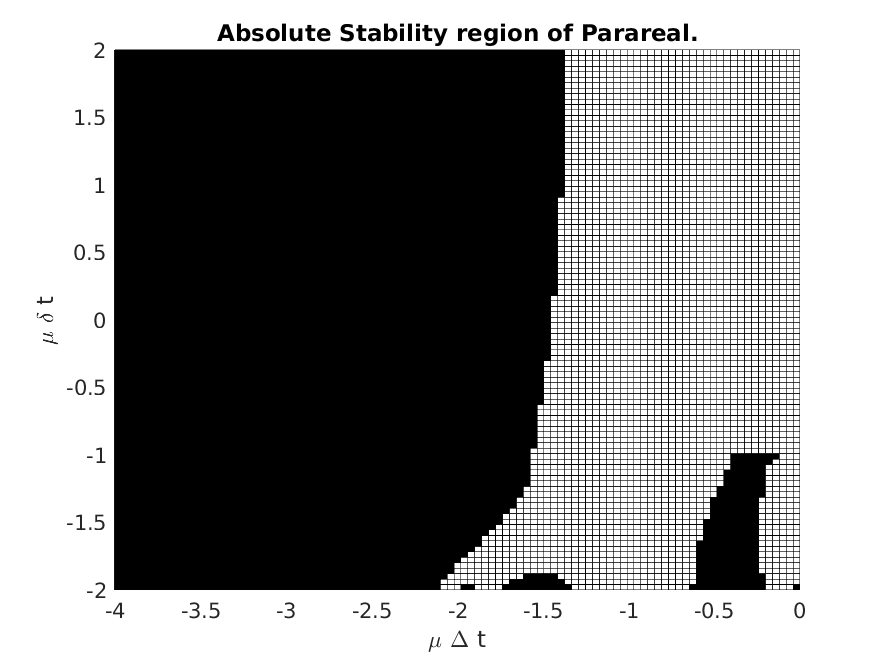
\includegraphics[width=.8\textwidth]{./resources/stability_fw}
  \caption{}\label{fig:stability}
\end{figure}

\section{Convergence Analysis}

\section{Conclusion}

\clearpage
\addcontentsline{toc}{section}{Bibliography}
\begin{thebibliography}{9}
\bibitem{balarticle}
Bal.
\textit{On the Convergence and the Stability of the Parareal Algorithm to solve
Partial Differential Equations}.
Columbia University, APAM

\bibitem{fieldstalk}
Fields.
\textit{Parareal Methods}.
\url{http://www.cfm.brown.edu/people/jansh/page5/page10/page40/assets/Field_Talk.pdf}

\bibitem{levecue}
Levecue.
\textit{Finite Difference Methods for Ordinary and Partial Differential
  Equations}.
\url{https://epubs.siam.org/doi/abs/10.1137/1.9780898717839.fm}.

\bibitem{ruprecht}
Ruprecht.
\textit{A shared memory implementation of pipelined Parareal}.
DOI:10.1007/978-3-319-64203-1_48.

\bibitem{staff}
Staff and R{\o}nquist.
\textit{Stability of the Parareal Algorithm}.
Norweigian University of Science and Technology, Department of Mathematical
Sciences.


\end{thebibliography}



\end{document}
